\section{Applying Grad-CAM}
\nblink{nhs-chest-xray/analyze/grad-cam.ipynb}

An implementation of Grad-CAM is available in the Visual Attribution on GitHub \cite{visualattribution}. Visual Attribution is not available on PyPI, we therefore copied the relevant code into our own GitHub repository. Visual Attribution is built on top of PyTorch so the integration into our project was simple. Grad-CAM was run on the last layer before the linear (dense) output layer, which is a batch normalization layer. The output shape of a batch normalization layer that follows a convolutional layer is the same as the convolutional layer, Grad-CAM can therefore be applied on these too. We also tried running on the last real convolutional layer, with much worse results.

\subsection{Results}
\begin{figure}[H]
\centering
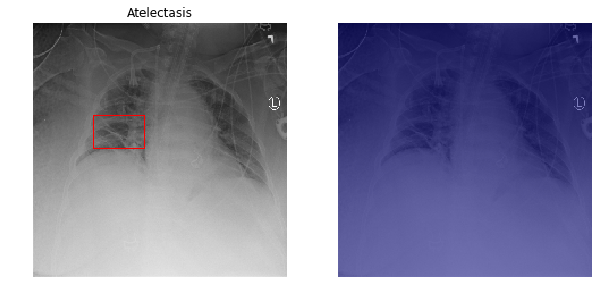
\includegraphics[width=12cm]{chapters/03_classification/images/grad-cam_0.png}
\caption{The left image shows the input image with the bounding box added by a physician. The right image shows the output of Grad-CAM, which in this case is blank.}
\label{grad_cam_example_1}
\end{figure}

\begin{figure}[H]
\centering
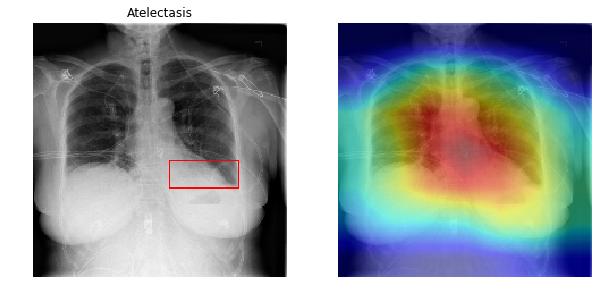
\includegraphics[width=12cm]{chapters/03_classification/images/grad-cam_2.png}
\caption{The left image shows the input image with the bounding box added by a physician. The right image shows the output of Grad-CAM which contains the bounding box in the region detected as important, but the region is much bigger and has the center outside of the bounding box.}
\label{grad_cam_example_2}
\end{figure}

\begin{figure}[H]
\centering
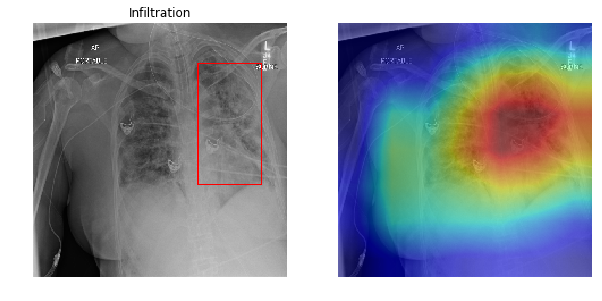
\includegraphics[width=12cm]{chapters/03_classification/images/grad-cam_8.png}
\caption{The left image shows the input image with the bounding box added by a physician. The right image shows the output of Grad-CAM. The center of the output matches the bounding box quite well.}
\label{grad_cam_example_3}
\end{figure}

\subsection{Discussion}
As seen in Figure \ref{grad_cam_example_1}, the output of Grad-CAM can be completely blank. This happens in 7 out of 21 tested images. The cause for this could not be found.

Other examples like \ref{ǵra

Looks ok, sometimes superpixels are completely missing



\subsection{Conclusion}